\section{连续性的判据}
\label{sec:mmap-continuity-criteria}

第~\ref{chap:topological-spaces}章用开集原像定义了连续映射，也把“在一点$x$连续”写成了邻域的语言：$f(x)$的每个邻域$V$，都对应$x$的某个邻域$U$，使$f(U)\subseteq V$。在度量空间中，邻域可以换成球，这句话就变成输入误差与输出误差之间的一句保证：输出精度要求多高，都能找到足够小的输入误差范围来满足它。

本节先写出这句保证，并证明它与开集定义一致，再用点列来检验连续性。度量空间中点列足以判断连续，一般拓扑空间里却只有单方向的结论，这一差别也放在本节说明。

本章固定记号：$(X,d_X)$与$(Y,d_Y)$是度量空间，$f:X\to Y$是映射；不致混淆时把两个度量都写作$d$。

\subsection{连续性的距离判据}
\label{sec:mmap-epsilon-delta}

先用一个具体函数走一遍。取$f(x)=x^2$，考察$x=1$处的误差。对任何输入$x'$，因式分解给出
\[
 \lvert x'^2-1\rvert=\lvert x'-1\rvert\,\lvert x'+1\rvert.
\]

先约定$\lvert x'-1\rvert<1$，这时$x'\in(0,2)$，第二个因子小于$3$。于是
\[
 \lvert x'^2-1\rvert<3\lvert x'-1\rvert.
\]

要把输出误差控制在$\varepsilon=0.1$以内，只要输入误差小于$0.1/3$。两个要求合起来，取
\[
 \delta=\min\Bigl\{1,\frac{0.1}{3}\Bigr\}=\frac1{30},
\]
则$\lvert x'-1\rvert<\delta$时$\lvert x'^2-1\rvert<0.1$。把$0.1$换成任意$\varepsilon>0$，$\delta=\min\{1,\varepsilon/3\}$同样可用。这就是下面这句保证的一个实例。

图~\ref{fig:mmap-epsilon-delta}把这句保证画成两个球。输出端先给定以$f(x)$为心、半径$\varepsilon$的球，要做的是在输入端找到一个足够小的球$B(x,\delta)$，使它的整个像都落在输出的球内。

\begin{BookInlineFigure}
  \centering
  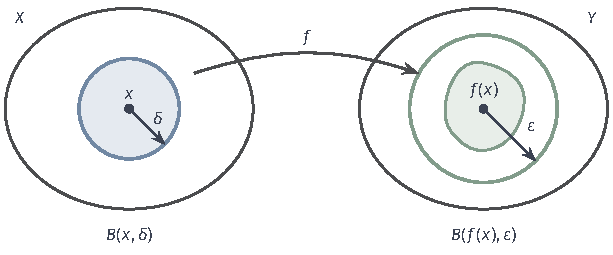
\includegraphics[width=103.738mm]{figures/04-spaces-measures-and-geometry/01-topology-and-metric/tikz/mmap-epsilon-delta/figure.pdf}
  \caption{一点连续的距离判据。蓝色球是输入端的$B(x,\delta)$，绿色圆是输出端的$B(f(x),\varepsilon)$，绿色填充区域是像$f(B(x,\delta))$。给定$\varepsilon$后，要找到足够小的$\delta$，使像完全落在绿色圆内；像本身不必是球。}
  \label{fig:mmap-epsilon-delta}
\end{BookInlineFigure}

把“$f(U)\subseteq V$”中的邻域都换成球，就得到熟悉的$\varepsilon$-$\delta$条件。

\begin{theorem}[一点连续的距离判据]
\label{thm:mmap-epsilon-delta}
$f$在$x\in X$处连续，当且仅当对任意$\varepsilon>0$，存在$\delta>0$，使得对所有$x'\in X$，
\begin{equation}
 d_X(x,x')<\delta
 \quad\Longrightarrow\quad
 d_Y(f(x),f(x'))<\varepsilon.
 \label{eq:mmap-epsilon-delta}
\end{equation}
\end{theorem}

\begin{proof}
设$f$在$x$处连续，给定$\varepsilon>0$。球$B(f(x),\varepsilon)$是$f(x)$的邻域，按一点连续的定义，有$x$的邻域$U$使
\[
 f(U)\subseteq B(f(x),\varepsilon).
\]
度量空间中$x$的邻域包含某个球，设$B(x,\delta)\subseteq U$。这个$\delta$满足式~\eqref{eq:mmap-epsilon-delta}。

反过来，设距离条件成立，$V$是$f(x)$的邻域。$V$包含某个球$B(f(x),\varepsilon)$，对这个$\varepsilon$取条件中的$\delta$，令$U=B(x,\delta)$。则$U$是$x$的邻域，并且
\[
 f(U)\subseteq B(f(x),\varepsilon)\subseteq V.
\]
所以$f$在$x$处连续。
\end{proof}

条件中的$\delta$可以依赖$x$，也可以依赖$\varepsilon$。它回答的问题是：输出允许的误差已经给定，输入需要控制在多小的范围内。前面的$x^2$例子里，$x=1$时用的是$\delta=\min\{1,\varepsilon/3\}$，换到别的点，这个公式就要跟着改变。

下一个定理说明，每一点都满足这句保证，恰好就是第~\ref{chap:topological-spaces}章定义的连续映射。

\begin{theorem}[逐点连续与开集原像]
\label{thm:mmap-pointwise-open-preimage}
$f$在$X$的每一点满足定理~\ref{thm:mmap-epsilon-delta}的距离条件，当且仅当$Y$中每个开集的原像都是$X$中的开集。
\end{theorem}

\begin{proof}
设距离条件处处成立，$U\subseteq Y$是开集，$x\in f^{-1}(U)$。$U$是开集，所以可取$\varepsilon>0$使$B(f(x),\varepsilon)\subseteq U$。再取对应的$\delta$，距离条件给出
\[
 f(B(x,\delta))\subseteq B(f(x),\varepsilon)\subseteq U,
\]
也就是$B(x,\delta)\subseteq f^{-1}(U)$。$x$是$f^{-1}(U)$中任意一点，所以$f^{-1}(U)$是开集。

反过来，设开集的原像都是开集。对$x\in X$和$\varepsilon>0$，集合$f^{-1}(B(f(x),\varepsilon))$是包含$x$的开集，所以其中有某个球$B(x,\delta)$。这个$\delta$满足式~\eqref{eq:mmap-epsilon-delta}。
\end{proof}

由$f^{-1}(Y\setminus F)=X\setminus f^{-1}(F)$，开集原像为开集等价于闭集原像为闭集，后者常用来判断集合是闭集。例如$g(\bm x)=x_1^2+x_2^2$在$(\mathbb R^2,d_2)$上连续，于是单位圆周是闭集，原因是
\[
 S^1=g^{-1}(\{1\}),
\]
单点集$\{1\}$是$\mathbb R$中的闭集；同样，圆盘$\{\bm x:g(\bm x)\leq4\}=g^{-1}((-\infty,4])$也是闭集。

连续性只保证原像保持开闭，不保证像保持开闭。$f(x)=x^2$把开区间$(-1,1)$映成$[0,1)$，后者在$\mathbb R$中不是开集，因为$0$处没有向左的邻域。$f(x)=e^x$把闭集$\mathbb R$映成$(0,\infty)$，后者不是闭集，因为$0$在它的闭包中。把开集映成开集的映射称为开映射，这是另一回事。

距离函数是最常用的连续函数。固定$z\in X$，由三角不等式$d(x,z)\leq d(x,x')+d(x',z)$，交换$x,x'$后合起来得到
\[
 \lvert d(x,z)-d(x',z)\rvert\leq d(x,x').
\]

对非空集合$A\subseteq X$，每个$a\in A$满足$d(x,A)\leq d(x,a)\leq d(x,x')+d(x',a)$。对$a$取下确界，再交换$x,x'$，得到
\[
 \lvert d(x,A)-d(x',A)\rvert\leq d(x,x').
\]

这两个函数都可以取$\delta=\varepsilon$，并且这个$\delta$对所有点通用，这种通用性下一节将命名为均匀连续。它们的零点集分别是$\{z\}$和$\overline A$，这再次说明单点集与闭包都是闭集。

\subsection{连续性的序列判据}
\label{sec:mmap-sequential-continuity}

对每个$\varepsilon$找$\delta$，有时不如直接看点列方便。上一章已经用点列描述了闭包，度量空间中点列同样足以探测连续性。

\begin{theorem}[连续性的序列判据]
\label{thm:mmap-sequential-continuity}
$f$在$x$处连续，当且仅当对$X$中每个满足$x_n\to x$的点列，都有$f(x_n)\to f(x)$。
\end{theorem}

\begin{proof}
设$f$在$x$处连续，$x_n\to x$。给定$\varepsilon>0$，取距离条件中的$\delta$，再取$N$使$n\geq N$时$d(x_n,x)<\delta$。这些$n$都满足
\[
 d(f(x_n),f(x))<\varepsilon,
\]
所以$f(x_n)\to f(x)$。

反方向用反证法。设$f$在$x$处不连续，按定理~\ref{thm:mmap-epsilon-delta}，存在某个$\varepsilon>0$，使任何$\delta>0$都不满足条件。对每个$n$取$\delta=1/n$，这一失败给出一点$x_n$，满足
\[
 d(x_n,x)<\frac1n,\qquad d(f(x_n),f(x))\geq\varepsilon.
\]
于是$x_n\to x$，而$f(x_n)$不趋于$f(x)$，与假设矛盾。
\end{proof}

序列判据特别适合否定连续性：只需找到一个趋于$x$、像却不趋于$f(x)$的点列。在$\mathbb R^2$上令
\[
 f(\bm x)=\frac{x_1x_2}{x_1^2+x_2^2}\quad(\bm x\neq\bm 0),\qquad f(\bm 0)=0.
\]

沿对角线上的点$\bm x_n=(1/n,1/n)$，分子是$1/n^2$，分母是$2/n^2$，于是
\[
 f(\bm x_n)=\frac12,\qquad \bm x_n\to\bm 0,
\]
像不趋于$f(\bm 0)=0$，所以$f$在原点不连续。沿坐标轴趋近时函数值恒为$0$，只看这个方向会得出错误结论：判据要求每一个趋于该点的点列都保持极限。

序列判据也可以用来肯定连续性。设$f:X\to Y$在$x$处连续，$g:Y\to Z$在$f(x)$处连续。若$x_n\to x$，则$f(x_n)\to f(x)$，再由$g$的连续性得
\[
 g(f(x_n))\to g(f(x)).
\]
所以$g\circ f$在$x$处连续。第~\ref{chap:topological-spaces}章已用开集原像证明了复合映射的连续性，这里是它在度量空间中的另一种读法。

在一般拓扑空间中，正方向仍然成立。若$f$连续且$x_n\to x$，对$f(x)$的邻域$V$，$f^{-1}(V)$是$x$的邻域，点列最终落在其中，所以$f(x_n)$最终落在$V$中。

反方向依赖于点列能否探测拓扑。上面的证明取$\delta=1/n$依次选点，用的正是每点有可数个球作邻域基；第~\ref{chap:topological-spaces}章的余可数拓扑没有这样的邻域基，那里给出了保持全部收敛点列、却不连续的映射。
